\documentclass[usenames,dvipsnames,10pt,aspectratio=169]{beamer} 
% Add option 'aspectratio=169' for 16:9 widescreen 
% Add option  'handout' to ignore animations
% If you have a smaller amount of text, feel free to also try '11pt'! / Jesper

\usepackage[utf8]{inputenc}
\usepackage{verbatim}
\usepackage{minted}
\usepackage{graphicx}
\usepackage{wrapfig}
\usepackage{geometry}
\usepackage{listings}
\usepackage{color, xcolor}
\usepackage[document]{ragged2e}
\usetheme{umu}

\usemintedstyle{monokai}

\usepackage{hyperref}
\hypersetup{
    colorlinks=true,
    linkcolor=ucugreyish,
    filecolor=ucured,
    urlcolor=ucublue,
}
\urlstyle{same}

\lstdefinestyle{codestyle}{
    backgroundcolor=\color{ucugrey2},
    commentstyle=\color{ucugrey3},
    keywordstyle=\color{codeblue},
    numberstyle=\tiny\color{codewhite},
    stringstyle=\color{codegreen},
    basicstyle=\ttfamily\small,
    breakatwhitespace=false,         
    breaklines=true,                 
    captionpos=b,                    
    keepspaces=true,                 
    numbers=left,                    
    numbersep=5pt,                  
    showspaces=false,                
    showstringspaces=false,
    showtabs=false,                  
    tabsize=2
}

%%% Some useful commands
% pdf-friendly newline in links
\newcommand{\pdfnewline}{\texorpdfstring{\newline}{ }} 
% Fill the vertical space in a slide (to put text at the bottom)
\newcommand{\framefill}{\vskip0pt plus 1filll}

%%% Enter additional packages below (or above, I can't stop you)! / Jesper
\renewcommand{\proofname}{\sffamily{Proof}}

% presentation template slides usage
% \framecard[color (not working)]{textbuf}
% \framesplit{Header}{picture}{textbuf}
% \framepic{image}{text}

%%%%%%%%%%%%%%%%%%%%%%%%%%%%%%%%%%%%%%%%%%%%%%%%%%%%%%%%%%%%%%%%%%%%%%%%%%%%%%%%%%%%%
\title{Linux course}
\subtitle{Shell}
\date[\today]{\small\today}
\author[Morhunenko Mykola]{Morhunenko Mykola}
\institute{APPS@UCU}

\begin{document}

\begin{frame}
\titlepage
\end{frame}

\begin{frame}{\contentsname}
\setbeamercolor{background canvas}{bg=ucugrey}
\tableofcontents
\end{frame}

\section{What Command Shell is?}
\framecard{What Command Shell is?}

\begin{frame}{What is command Shell?}
\begin{itemize}
    \item Command Shell is a computer program, that provide the user with a (CLI) command line interface to control the computer using keyboard, without GUI (Graphical user interface), for communication with the Linux system
    \item If you are using Linux, you have definitely see the command prompt. Usually it looks like {\color{ucugreen}\$} or, probably, {\color{ucugreen} \text{[username@hostname path] }\$}
    \item From the very beginning it looks like GUI is faster, but it is totally false: CLI just have high entry threshold. But it allows to write scripts (files with shell commands) that can automate routine, which is impossible in GUI
    \item Much more programs provide only CLI. If you want to use servers, connect to other computers via ssh, to be a real programmer, you must know shell
    \item You can check your shell by the command {\color{ucugreen} \$ echo \$SHELL}
    \item Most likely you have {\color{ucugreen} bash}, the most popular and stable one
    \item If you are done, you can leave the shell with {\color{ucugreen} exit} command, or by pressing the {\color{ucugreen}Ctrl+d} in the terminal emulator window
\end{itemize}
\end{frame}

\begin{frame}{What is Bash}
\begin{itemize}
    \item Bash stands for "Bourne(born)-again-shell"
    \item It is default shell for most Linux distros
    \item POSIX standard have a full description of the shell. Bash implements all this features, plus something own, known as {\color{ucugreen} bashism}
    \item Bash is a standard shell for the majority of  Linux distros, but it doesn't mean it is the best one
\end{itemize}
\end{frame}

\begin{frame}{ZSH}
    \begin{itemize}
        \item Zsh stands for {\color{ucugreen}Z-shell}
        \item Like Bash, it derives from Bourne family of shells, in everyday usage zsh is the same, as {\color{ucugreen} bash}, but have a lot of extensions and other syntax of configuration files (default - {\color{ucugreen}~/.zshrc})
        \item There is an entire eco-system of configuration tools and themes called oh-my-zsh which is very popular
        \item Also there are a huge amount of extensions at the github, that can make everyday usage easier - from auto-complete to syntax highlighting
        \item also there are differences in scripts, about it is later.
        
    \end{itemize}
\end{frame}


\section{Paths}
\framecard{Paths}
\begin{frame}{Path}
    \begin{itemize}
        \item  {\color{ucugreen} Path} - one of the most important terms in this topic (and in understanding, how programs work)
        \item Current path - or current directory, working directory - the directory, from where you are working, launching programs/scripts
        \item Paths can be absolute or relative
        \item Absolute
            \begin{itemize}
                \item {\color{ucugreen} /} - also known as  {\color{ucugreen} root path}, all paths that starts from it are {\color{ucugreen} absolute}. Other examples:
                \item {\color{ucugreen} /home/username}
                \item {\color{ucugreen} /usr/local/share/zsh/site-functions/}
            \end{itemize}
        \item Relative
            \begin{itemize}
                \item Relative paths don't starts from the root. Shell interpreter always run all programs with respect to the current path. They never begins with \ex{/}
                \item {\color{ucugreen} .zshrc}
                \item {\color{ucugreen} Documents/UCULinux/presentations}
            \end{itemize}
    \end{itemize}
\end{frame}
\begin{frame}{Path}
    \begin{itemize}
        \item Names are case-sensitive, that means {\color{ucugreen} /home/UserName} and {\color{ucugreen} /home/username} are different names
        \item There are also special paths
        \begin{itemize}
            \item {\color{ucugreen} ./} stands for the current path
            \item {\color{ucugreen} ../} stands for the path one step back. For example, if the {\color{ucugreen} ./} is {\color{ucugreen} /home/username}, the {\color{ucugreen} ../} will be {\color{ucugreen} /home}
            \item {\color{ucugreen} \textasciitilde /} stands for the directory of current user. For example, for {\color{ucugreen} root} user {\color{ucugreen} ~/} will be {\color{ucugreen} /root}, and for {\color{ucugreen} username} it will be {\color{ucugreen} /home/username}
        \end{itemize}
    \end{itemize}
\end{frame}

% \section{Bash Intro}
% \framecard{Bash Intro}

% \begin{frame}{Syntax}
%     All default commands (programs) have very similar syntax
%     \begin{examples}
%     \text{program\_name [option]... [arguments]...}
%     \end{examples}
%     Options starts from \ex{-} or \ex{-{}-} \newline
%     To see, how to use any command
%     \begin{examples}
%         \text{program\_name -h} \newline or
%         \text{program\_name -{}-}help \newline behind are synonyms, but parameter is in short and long form \newline
%         man \text{program\_name}  - it provides full documentation about the command
%     \end{examples}
% \end{frame}

% \begin{frame}{Base commands}
% \begin{itemize}
%     \item \ex{pwd} - print working directory - show your current path
%     \item \ex{ls <path>} - list - show what is inside the directory
%     \item \ex{cd [path]} - change directory - change your current directory
% \end{itemize}
% So now it is possible to get something 
% \begin{examples}
%     username\$ pwd \newline
%     \ex[ucugrey]{> /home/username} \newline
%     username\$ ls \newline
%     \ex[ucugrey]{> Desktop Documents Downloads Music Pictures Videos} \newline
%     username\$ cd Downloads \newline
%     username\$ pwd \newline
%     \ex[ucugrey]{> /home/username/Downloads}
% \end{examples}
% \end{frame}
% \begin{frame}{Base commands}

% {\Large{Introducing ls}} \newline
% \begin{itemize}
%     \item \ex{ls -a} - list all, including names starting with dot symbol "."
%     \item \ex{ls -l} - list using a long list format, to display more information including permissions, size and important dates
%     \item \ex{ls -r} - list in reversed order
%     \item \ex{ls -R} - list current directory and all subdirectories recursively
%     \item \ex{ls -S} - sort by file size, largest first
%     Also they can be combined. The most commonly used
%     \item \ex{ls -la} - list all with full info
%     And the command have path as an argument, so the following command is also valid
%     \item \ex{ls -la /etc/systemd/system}
% \end{itemize}
% And there are much more options, that can be found using \ex{ls -{}-help}
% \end{frame}

% \begin{frame}{Base commands}
%     Now you can move around and see, what is around. But to work on your labs or projects, you need to create something and see, what is inside, and somehow manipulate it: \newline
%     \begin{itemize}
%         \item \ex{mkdir [dirname]} - make directory - create a new directory
%         \item \ex{touch [filename]} - create a file with filename or update the date of file's last modification to current date
%         \item \ex{date} - print current date and time
%         \item \ex{echo [text]} - print the text to the standard output
%         \item \ex{cat [filename]} - short for concatenate - show the file content
%         \item \ex{cp [source...] [destination]} - copy - copy all from source (all arguments except the last) to the destination (the last argument). \ex{-r} option required for directories
%         \item \ex{mv [source...] [destination]} - move - move all from source to destination
%         \item \ex{rm [path]} - remove - remove the file. \ex{-rf} required for directories
%     \end{itemize}
% \end{frame}

% \begin{frame}{Going deeper}

%     {\Large Creating Links} \newline
%     In Linux there are two types of links: hard and symbolic
%     \begin{itemize}
%         \item Inode - a data structure in the Unix-style file systems, that describes a file-system object
%         \item Inode can have any number of hard links, and the inode will persists on the system until all hard links disappear. Changing in one file apply this changes also to all it's hard links
%     \end{itemize}
% \end{frame}

% \begin{frame}{Going deeper}
%     \begin{itemize}
%         \item \ex{ls -i} command is used to list all files with it's inodes
%         \item \ex{ln [source] [destination]} is used to create hard links
%         \begin{examples}
%             username \$ ln file1 file2 \newline
%             username \$ ls -i \newline
%             \ex[ucugrey]{> 9700529 file1  9700529 file2}
%         \end{examples}
%         as far as wee can see, both files have same inode
%         \begin{examples}
%         username \$ echo "Hello Wrold!" >> file1 \newline
%         username \$ cat file2 \newline
%         \ex[ucugrey]{> Hello World!}
%         \end{examples}
%         So changes in one file apply this changes to the other one \newline
%     \end{itemize}
% \end{frame}

% \begin{frame}{Going deeper}
%     What about symbolic links?
%     \begin{itemize}
%         \item symbolic links (symlinks) are used more often. This is a special type, and the link refers to another file by name, not by inode.
%         \item deleting the source file will make the symlink broken
%         \item \ex{ln -s} - used to create the symbolic link
%         \begin{examples}
%         username \$ ln -s file1 file3 \newline
%         username \$ ls -l \newline
        
%         > -rw-rw-r-- 2 username groupname 18 Apr 17 00:47 file1 \newline
%         \, \, -rw-rw-r-- 2 username groupname 18 Apr 17 00:47 file2 \newline
%         \, \, lrwxrwxrwx 1 username groupname  5 Apr 17 00:54 file3 -> file1
%         \end{examples}
%         \item Symlinks can be created to any type of file system objects
%         \item Can be used to point to an object from another file system
%     \end{itemize}
% \end{frame}

% \begin{frame}{Going deeper}

%     {\Large Wildcards, Globs}
%     \begin{itemize}
%         \item In case, there is a folder with 25 test files, but it is necessary to delete first 8 of them... there are few ways, how to deal with that
%         \begin{examples}
%         username \$ rm test1 test2 test3 test4 test5 test6 test7 test8 \newline
%         \,\,\,or... \newline
%         username \$ rm test[1-8] \newline
%         \,\,\,or if you want to delete all tests... \newline
%         username \$ rm test*
%         \end{examples}
%         \item So, \ex{*} wildcard stands for all matches, any number of any symbol
%         \item \ex{?} stands for \ex{any one symbol}
%         \item \ex{[]} wildcard stands for ranges, so \ex{[abc]} means "any of a, b, c", the same for [a-c]
%         \item \ex{!} stands for non-match, so [!a] stands for any symbol except 'a'
%     \end{itemize}
% \end{frame}

% \begin{frame}{Going deeper}

%     {\Large Important about wildcards}
%     \begin{itemize}
%         \item Be careful while using wildcards
%         \item Bash preprocess all input to extend it with respect to wildcards
%         \item so if you want to use one of such symbols just as symbols, you can either escape character with \ex{\textbackslash} symbol, or use single quotes
%         \begin{examples}
%         username \$ echo [fo]* > ./new\_file \newline in this case you will add names of all files starts with 'f' or 'o' \newline
%         username \$ echo '[fo]*' > ./new\_file\newline
%         username \$ echo \textbackslash [fo\textbackslash ]\textbackslash * > ./new\_file \newline
%         both approaches above are correct
%         \end{examples}
%         \item \ex{ All bash commands are \href{https://ss64.com/bash/}{here}}
%     \end{itemize}
% \end{frame}

% \begin{frame}{Searching}
%     \begin{itemize}
%         \item So as for now we know how to create files, directories, move them and remove. But how to find them?
%         \item The Linux file system is well-structured, so it's very easy to navigate it, but still there are thousands of files and it's impossible to remember all locations. About the Linux File system hierarchy there is entire presentation
%         \item \ex{find [path] -name ["filename"]}, and in the name can globs can be used (but they must be escaped)
%         \item But if you don't know for sure the filename or dirname, the better way is \ex{find <path> -regex ["filename\_regex"]}
%         \item \ex[ucured]{Be careful!} All files in the system have own permissions. So to search somewhere outside the \ex{/home/username} folder, you must run the program in privileged mode
        
%     \end{itemize}
% \end{frame}

% \section{Permissions}
% \framecard{Permissions}

% \framesplitc{Extensions}{graphics/ext.jpg}{
%     \begin{itemize}
%         \item The Linux world doesn't need file extensions
%         \item The operating system doesn't use them to determine how to open a file
%         \item But extensions are used by some parts of the OS to determine which program to use to open file
%         \item So how the operating system find out, what the file is and how to deal with it?
%     \end{itemize}
% }

% \begin{frame}{Permissions}
%     \begin{itemize}
%         \item When executing the \ex{ls -l} command, at the very beginning of every line there is 10 characters and then two words
%         \begin{examples}
%         username \$ ls -la \newline
%         \ex[ucugrey]{> drwxrwxr-x 10 username groupname 4096 Apr 20 02:21 example\_directory} \newline
%         \ex[ucugrey]{\,\,\, -rw-rw-r-{}- \hspace{0.2cm} 10 username groupname 4096 Apr 20 02:21 example\_textfile} \newline
%         \ex[ucugrey]{\,\,\, -rwxr-xr-x \hspace{0.25cm} 10 username groupname 4096 Apr 20 02:21 example\_binary\_file} \newline
%         \end{examples}
%         \item They are not just letters, there is a lot of information behind these 10 characters (or, actually, 3 decimal numbers)
%     \end{itemize}
% \end{frame}

% \begin{frame}{Permissions}
%     \begin{figure}
%         \centering
%         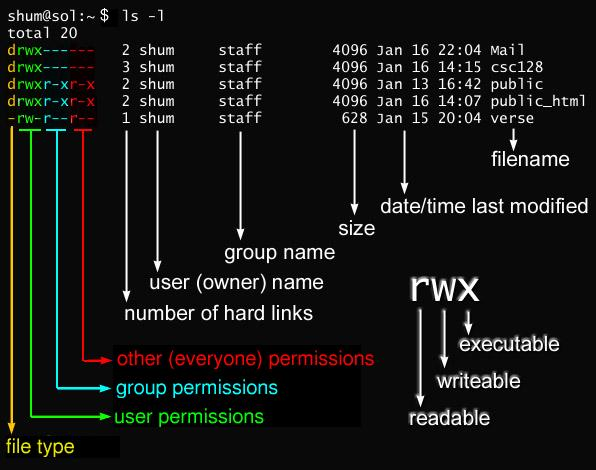
\includegraphics[height=0.8\paperheight]{graphics/permissions1.jpg}
% \end{figure}
    
% \end{frame}


% \framesplitc{Permissions}{graphics/permissions.png}{
%     \begin{itemize}
%         \item The very first letter stands for file type (about them the info will be in the File systems topic)
%         \item To change permissions, there is a command \ex{chmod}
%         \item To see all possible parameters, use \ex{chmod -{}-help}. (But some explanations for the beginners are on the next page)
%         \item All triplets of permissions \ex{rwx} have it's number correspondences
%     \end{itemize}
% }

% \begin{frame}{Permissions}
%     \begin{itemize}
%         \item So in the help of \ex{chmod} are a little bit confusing things
%         \item In \ex{[ugoa]} - User, Group, Other users, All
%         \item In \ex{[rwxXst]} - Read, Write, eXecute
%         \item eXecute only if the file is a directory or already has execute permission for some user
%         \item Set user or group ID on execution
%         \item Save program text on swap device (a performance enhancer)
%     \end{itemize}
% \end{frame}

% \framesplitc{Sudo}{graphics/sudo_meme.jpg}{
%     \begin{itemize}
%         \item By default, every user have permissions to play around only his \ex{/home/username} directory
%         \item To somehow modify the system (either install programs or modify global settings), you need so named \ex{superuser mode}
%         \item If have the error starting with \ex[ucured]{permission denied}, them you need to run the program with privilages, for example, using \ex{sudo}
%     \end{itemize}
% }

% \framesplitc{Sudo}{graphics/password_meme.jpg}{
%     \begin{itemize}
%         \item To run any program as superuser, use \ex{sudo <program\_name> <program\_parameters>}, sudo stands for "super user do"
%         \item To login the shall as a superuser, both \ex{su root} and \ex{sudo -i} can be used. \ex[ucured]{When you type a password, it stays invisible}
%         \item \ex[ucured]{\large DO NOT RUN GUI AS ROOT!} instead use \ex{gksu} (it is deprecated for as 2021, but still in AUR) or alternatives (\ex{kdesu, sux})
    
%     \end{itemize}
% }

% \section{Scripts}
% % redirections, variables etc.
% \framecard{Scripts}

% \begin{frame}{Scripts}
%     \begin{itemize}
%         \item Script - just file with bunch of commands that can be interpreted (e.g. python, lisp scripts, or bash scripts)
%         \item They can be used both for automation some small routine tasks and as large programs
%         \item Shell scripts names ends with \ex{.bash}, \ex{.sh}, \ex{zsh}
%         \item But as far as we know, the Linux system doesn't use the extensions to identify the type of file. So how to run a script as a usual program?
%         \item One of possible ways to run the script - give it as a parameter to the command interpreter
%         \begin{examples}
%             username \$ bash ./my\_first\_script.sh \newline
%             \ex[ucugrey]{> some output}
%         \end{examples}
%     \end{itemize}
% \end{frame}

% \begin{frame}{Scripts}
%     \begin{itemize}
%         \item Or we can make the file executable (add \ex{x} or \ex{111} flag)
%         \begin{examples}
%             username \$ chmod +x ./my\_first\_script \newline
%             username \$ ./my\_first\_script \newline
%             \ex[ucugrey]{some output}
%         \end{examples}
%         \item But, actually, there is a mistake. If do it in the following way, the script will be run from the running shell. But we want to make Python, Ruby. Scheme also executable. Unfortunately, the bash interpreter can not execute them...
%     \end{itemize}
% \end{frame}

% \begin{frame}{Shebang}
%     \begin{itemize}
%         \item \ex{\large Shebang} - the name of the character sequence at the very first line of the script (\ex[ucured]{line \#1, that is important!}) that specify the absolute path to the interpreter.
%         \lstinputlisting[language=Bash, style=codestyle]{code/shebang_ex.sh}
%         \item Or also possible variant (to search for the interpreter in PATH (about PATH in next presentation))
%         \lstinputlisting[language=Python, style=codestyle]{code/shebang_ex.py}
%     \end{itemize}
% \end{frame}

% \begin{frame}{Variables}
%     \begin{itemize}
%         \item  User can define and use variables at the environment:
%         \begin{examples}
%             username \$ my\_var="This is my var"
%         \end{examples}
%         \item \ex[ucured]{There is no space on either side of the "=" sign allowed}
%         \item There are local and global variables
%         \item When we "export" the var, it becomes available in all applications run from the current session, that means global 
%         \item For programs run from the shell, global variables are same as environment variables
%         \item To get the variable, \$\{\} syntax is used:
%         \begin{examples}
%             username \$ echo \$\{my\_var\} \newline
%             \ex[ucugrey]{> This is my var}
%         \end{examples}
%     \end{itemize}
% \end{frame}

% \begin{frame}{Script arguments}
%     \begin{itemize}
%         \item Scripts (actually, all programs) are useless without some input from the user
%         \item Just to remember, the default program calling syntax:
%         \begin{examples}
%             \text{program\_name [option]... [arguments]...}
%         \end{examples}
%         \item So to access the arguments:
%         \begin{itemize}
%             \item \ex{\$\{@\}} - all arguments
%             \item \ex{\$\{\#\}} - number (length) of all arguments
%             \item \ex{\$\{0\}} - script name
%             \item \ex{\$\{1\}}, \ex{\$\{2\}}... - other script parameters
%         \end{itemize}
%     \end{itemize}
% \end{frame}

% \begin{frame}{Quoting}
%     \begin{itemize}
%         \item As far as there are a lot of special characters, how to use them if you want to print it?
%         \item Quoting or escaping is used to make regular symbol from special one
%         \item \ex{\textbackslash} is used in a lot of programming languages
%         \begin{examples}
%             username \$ echo \$\{SHELL\} \newline
%             \ex[ucugrey]{/bin/zsh} \newline
%             username \$ echo \textbackslash\$\{SHELL\} \newline
%             \ex[ucugrey]{\$SHELL} 
%         \end{examples}
%         \item \ex{'} - single quotes, make "escaped" everything inside
%         \item \ex{"} - double quotes, allows variables expansion
%     \end{itemize}
% \end{frame}

% \begin{frame}{Conditionals. If}
%     \begin{itemize}
%         \item The standard \ex{if} with both one and many branches
%         \lstinputlisting[language=Bash, style=codestyle]{code/if_syntax.sh}
%         \item Example:
%         \lstinputlisting[language=Bash, style=codestyle]{code/conditions_ex.sh}
%     \end{itemize}
% \end{frame}

% \begin{frame}{Conditionals}
%     \begin{itemize}
%         \item There are a lot of conditions regarding different types:
%         \item For numbers:
%         \begin{itemize}
%             \item \ex{-lt} - <
%             \item \ex{-gt} - >
%             \item \ex{-le} - <=
%             \item \ex{-ge} - >=
%             \item \ex{-eq} - ==
%             \item \ex{-ne} - !=
%         \end{itemize}
%         \item Logical operations
%         \begin{itemize}
%             \item \ex{-a} - and
%             \item \ex{-o} - and
%             \item \ex{!} - not
%         \end{itemize}
%     \end{itemize}
% \end{frame}

% \begin{frame}{Conditionals}
%     \begin{itemize}
%         \item \ex{[-d FILE]} - True if FILE exists and is a directory
%         \item \ex{[-e FILE]} - True if FILE exists
%         \item \ex{[-f FILE]} - True if FILE exists and is a regular file
%         \item \ex{[-r FILE]} - True if FILE exists and is readable
%         \item \ex{[-s FILE]} -  True if FILE exists and has a size greater than zero
%         \item \ex{[-w FILE]} - True if FILE exists and is writable.
%         \item \ex{[-x FILE]} -  True if FILE exists and is executable
%         \item \ex{[-z STRING]} - True of the length if ”STRING” is zero
%         \item \ex{[-n STRING]} - True if the length of ”STRING” is non-zero
%         \item But for strings the most popular cooperators are used
%         \item \ex{[STRING1 == STRING2]} 
%         \item the same about <, >, !=, etc
%     \end{itemize}
% \end{frame}

% \begin{frame}{Conditionals. Case}
%     \begin{itemize}
%         \item If you have an experience in other programming languages, you definitely know the case statement. Here is the example:
%         \lstinputlisting[language=Bash, style=codestyle]{code/case_ex.sh}
%     \end{itemize}
% \end{frame}

% \begin{frame}{Loops}
%     If you know any programming language, you definitely know, what is loop. Here is bash syntax for them
%     \lstinputlisting[language=Bash, style=codestyle]{code/for_syntax.sh}
%     \lstinputlisting[language=Bash, style=codestyle]{code/while_syntax.sh}
%     \lstinputlisting[language=Bash, style=codestyle]{code/until_syntax.sh}
% \end{frame}

% \begin{frame}{Loop examples}
%     \lstinputlisting[language=Bash, style=codestyle]{code/for_ex.sh}
%     \lstinputlisting[language=Bash, style=codestyle]{code/while_ex.sh}
% \end{frame}

% \begin{frame}{More \ex{for loop} examples}
%     \lstinputlisting[language=Bash, style=codestyle]{code/for_extended_ex.sh}
% \end{frame}

% \begin{frame}{Arithmetic}
%     \begin{itemize}
%         \item In bash arithmetic is a little bit tricky
%         \item To evaluate the arithmetic expression, \ex{let} can can be used
%         \begin{examples}
%             username \$ a=4+5 \newline
%             username \$ echo \$a \newline
%             \ex[ucugrey]{> 4+5} \newline
%             username \$ a=((4+5)) \newline
%             username \$ echo \$a \newline
%             \ex[ucugrey]{> 9}
%         \end{examples}
%         \item \ex{+, -, *, /, ** (power), \%, ++, --} commands can be used 
%     \end{itemize}
% \end{frame}

% \section{Extended Bash}
% % pipes, grep (about regexp and entire lesson about it)
% \framecard{Extended Bash}

% \begin{frame}{Redirections}
    
% \end{frame}

% \begin{frame}{Pipes}
    
% \end{frame}

% \section{Sources}
% \framecard{The end =)}
% \framecard{Sources}
% \begin{frame}{Sources}
% \begin{itemize}
%     \item \href{https://cms.ucu.edu.ua/pluginfile.php/181565/mod_resource/content/3/os_p01_bash.pdf}{Bash presentation for Operating systems course, UCU, Oleg Farenyuk (only from UCU domain)}
%     \item \href{https://www.funtoo.org/Linux_Fundamentals,_Part_1}{Linux basics from the founder of Gentoo, Daniel Robbins, Chris Houser, Aron Griffis}
%     \item \href{https://www.funtoo.org/Bash_by_Example,_Part_1}{Bash basics, Daniel Robbins, Chris Houser, Aron Griffis}
%     \item \href {https://scriptingosx.com/}{Scripting OS X}
% \end{itemize}    
% \end{frame}

\end{document}